\documentclass[border=0pt]{standalone}
\usepackage{pgfplots}
%\pgfplotsset{width=7cm,compat=1.8}
\usepackage{pgfplotstable}
\renewcommand*{\familydefault}{\sfdefault}
\usepackage{sfmath}
%\pgfplotsset{width=7cm,compat=1.8}
%\usetikzlibrary{positioning, arrows, shapes, shadows, calc, fit}
%\usepackage{pgfplots}
%\usepackage{subcaption}


\begin{document}
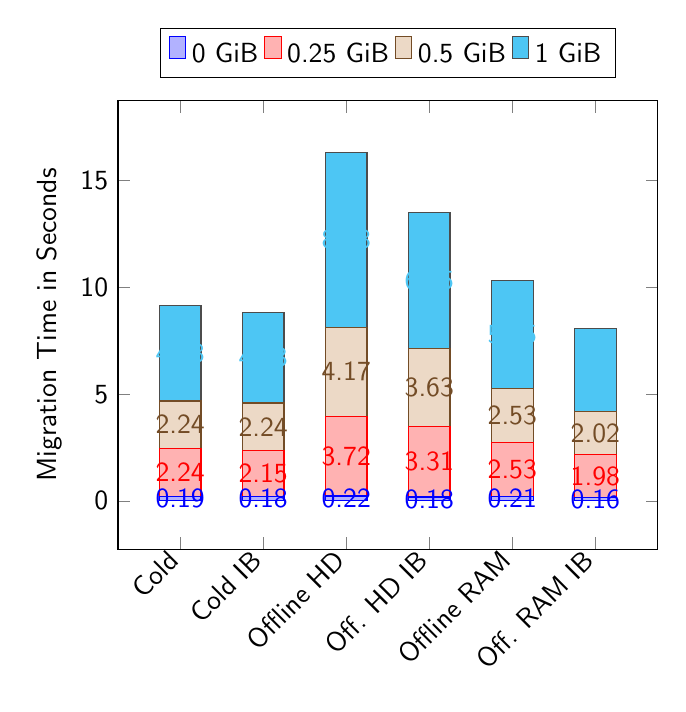
\begin{tikzpicture}
\begin{axis}[
ybar stacked,
bar width=15pt,
nodes near coords,
enlargelimits=0.15,
legend style={at={(0.5, 1.05)},
	anchor=south,legend columns=-1},
ylabel={Migration Time in Seconds},
symbolic x coords={Cold, Cold IB, Offline HD, Off. HD IB, 
	Offline RAM, Off. RAM IB},
xtick=data,
x tick label style={rotate=45,anchor=east},
]
\addplot+[ybar] plot coordinates {(Cold,0.1882) (Cold IB,0.1843) 
	(Offline HD,0.2238) (Off. HD IB,0.1778) (Offline RAM,0.2133) (Off. RAM IB,0.1638)};
\addplot+[ybar] plot coordinates {(Cold,2.2425) (Cold IB,2.1509) 
	(Offline HD,3.7215) (Off. HD IB,3.3126) (Offline RAM,2.5265) (Off. RAM IB,1.9847)};
\addplot+[ybar] plot coordinates {(Cold,2.2426) (Cold IB,2.2428)
	(Offline HD,4.1745) (Off. HD IB,3.6341) (Offline RAM,2.5285) (Off. RAM IB,2.0222)};
\addplot+[ybar, cyan!70, draw= black!70] plot coordinates {(Cold,4.4831) (Cold IB,4.2259) 
	(Offline HD,8.1813) (Off. HD IB,6.3509) (Offline RAM,5.0494) (Off. RAM IB,3.8975)};
\legend{\strut 0 GiB, \strut 0.25 GiB, \strut 0.5 GiB, \strut 1 GiB}
\end{axis}
\end{tikzpicture}
\end{document}